% Gemini theme
% https://github.com/anishathalye/gemini

\documentclass[final]{beamer}

% ====================
% Packages
% ====================

\usepackage[T1]{fontenc}
\usepackage{lmodern}
\usepackage[orientation=portrait,size=a0,scale=1.15]{beamerposter}
\usetheme{gemini}
\usecolortheme{gemini}
\usepackage{graphicx}
\usepackage{subcaption}
\graphicspath{{../common/personas}{../common/}{images}}
\usepackage{booktabs}
\usepackage{tikz}
\usepackage{pgfplots}
\pgfplotsset{compat=1.14}
\usepackage{anyfontsize}
\usepackage{smartdiagram}
\usesmartdiagramlibrary{additions}

% ====================
% Lengths
% ====================

% If you have N columns, choose \sepwidth and \colwidth such that
% (N+1)*\sepwidth + N*\colwidth = \paperwidth
\newlength{\sepwidth}
\newlength{\colwidth}
\newlength{\bigcolwidth}
\setlength{\sepwidth}{0.025\paperwidth}
\setlength{\colwidth}{0.45\paperwidth}
\setlength{\bigcolwidth}{0.925\paperwidth}

\newcommand{\separatorcolumn}{\begin{column}{\sepwidth}\end{column}}

% pandoc provides this command for lists
\newcommand{\pandocbounded}[1]{#1}
\providecommand{\tightlist}{%
  \setlength{\itemsep}{0pt}\setlength{\parskip}{0pt}}

% ====================
% Title
% ====================

\title{Standalone device for personal organization}
\author{
  Mason~Becker
  \and
  Sulaiman~Islam
  \and
  Isabella~Phung
  \and
  Akanksha~Rajagopalan
  \and
  Lennan~Tuffy
}
\institute[UC Santa Cruz]{CSE 123 - Supervised by Prof. David Harrison}
\date{\today}

% ====================
% Footer (optional)
% ====================

\footercontent{
  \href{https://engineering.ucsc.edu}{https://engineering.ucsc.edu} \hfill
  Senior Design Showcase 2025, UC Santa Cruz \hfill
  % FIXME who's contact info will we use?
  \href{mailto:ltuffy@ucsc.edu}{ltuffy@ucsc.edu}}
% (can be left out to remove footer)

% ====================
% Logo (optional)
% ====================

% use this to include logos on the left and/or right side of the header:
% \logoright{\includegraphics[height=7cm]{logo1.pdf}}
\logoright{
\includegraphics[height=7cm]{BE_Logomark_CMYK_color.pdf}}
% \logoleft{\includegraphics[height=7cm]{logo2.pdf}}

% ====================
% Body
% ====================

\begin{document}

\begin{frame}[t]
  \begin{columns}[t]
    \separatorcolumn

    % ====================
    % Begin column 1
    % ====================
    \begin{column}{\colwidth}

      \begin{block}{Abstract}
        % goal and need statment, remade to fit the poster presentation's context
        % required about 150+ words
        \begin{enumerate}
          \item \textbf{Presence:} Balanced between annoying and unnoticeable
          \item \textbf{Configurable:} Integration with existing productivity tools ex: Google Calendar
          \item \textbf{Accessible:} Easy to use and has data backup in case of device failure.
        \end{enumerate}
        \begin{itemize}
          \item \textbf{Simultaneous Tasks:} Up to 100
          \item \textbf{Price:} <\$100
          \item \textbf{Devices per user:} Unlimited
        \end{itemize}
      \end{block}

      \begin{block}{Personas} 
    
    \begin{minipage}[t]{0.3\linewidth}
      \centering
      \includegraphics[width=0.8\linewidth]{camillia.png}
    \end{minipage}
    \hfill
    \begin{minipage}[t]{0.65\linewidth}
      \textbf{Camillia - Cardiologist}
      
      Cardiologist, wants to balance demanding work schedule with quality time with kids. Needs help organizing daily tasks so that she can make it to special occasions with her family.
    \end{minipage}
    
    \vspace{0.5cm}
    
    \begin{minipage}[t]{0.3\linewidth}
      \centering
      
\includegraphics[width=0.8\linewidth]{Elijah.png}
    \end{minipage}
    \hfill
    \begin{minipage}[t]{0.65\linewidth}
      \textbf{Elijah - IT receptionist}
      
      [IT receptionist, wants to keep track of all the message assignments and dynamically edit his schedule to adapt to meeting times. Is married and wants to spend time with adopted puppy.]
    \end{minipage}
    
    \vspace{0.5cm}
    
    \begin{minipage}[t]{0.3\linewidth}
      \centering
      
\includegraphics[width=0.8\linewidth]{Linda.png}
    \end{minipage}
    \hfill
    \begin{minipage}[t]{0.65\linewidth}
      \textbf{Linda - Marketing and Sales}
      
      [Is striving for managerial position but often struggles to find time to let loose and rest.]
    \end{minipage}

  \end{block}

      \begin{block}{System Architecture}
      \begin{figure}
        \begin{subfigure}[t]{0.54\textwidth}
            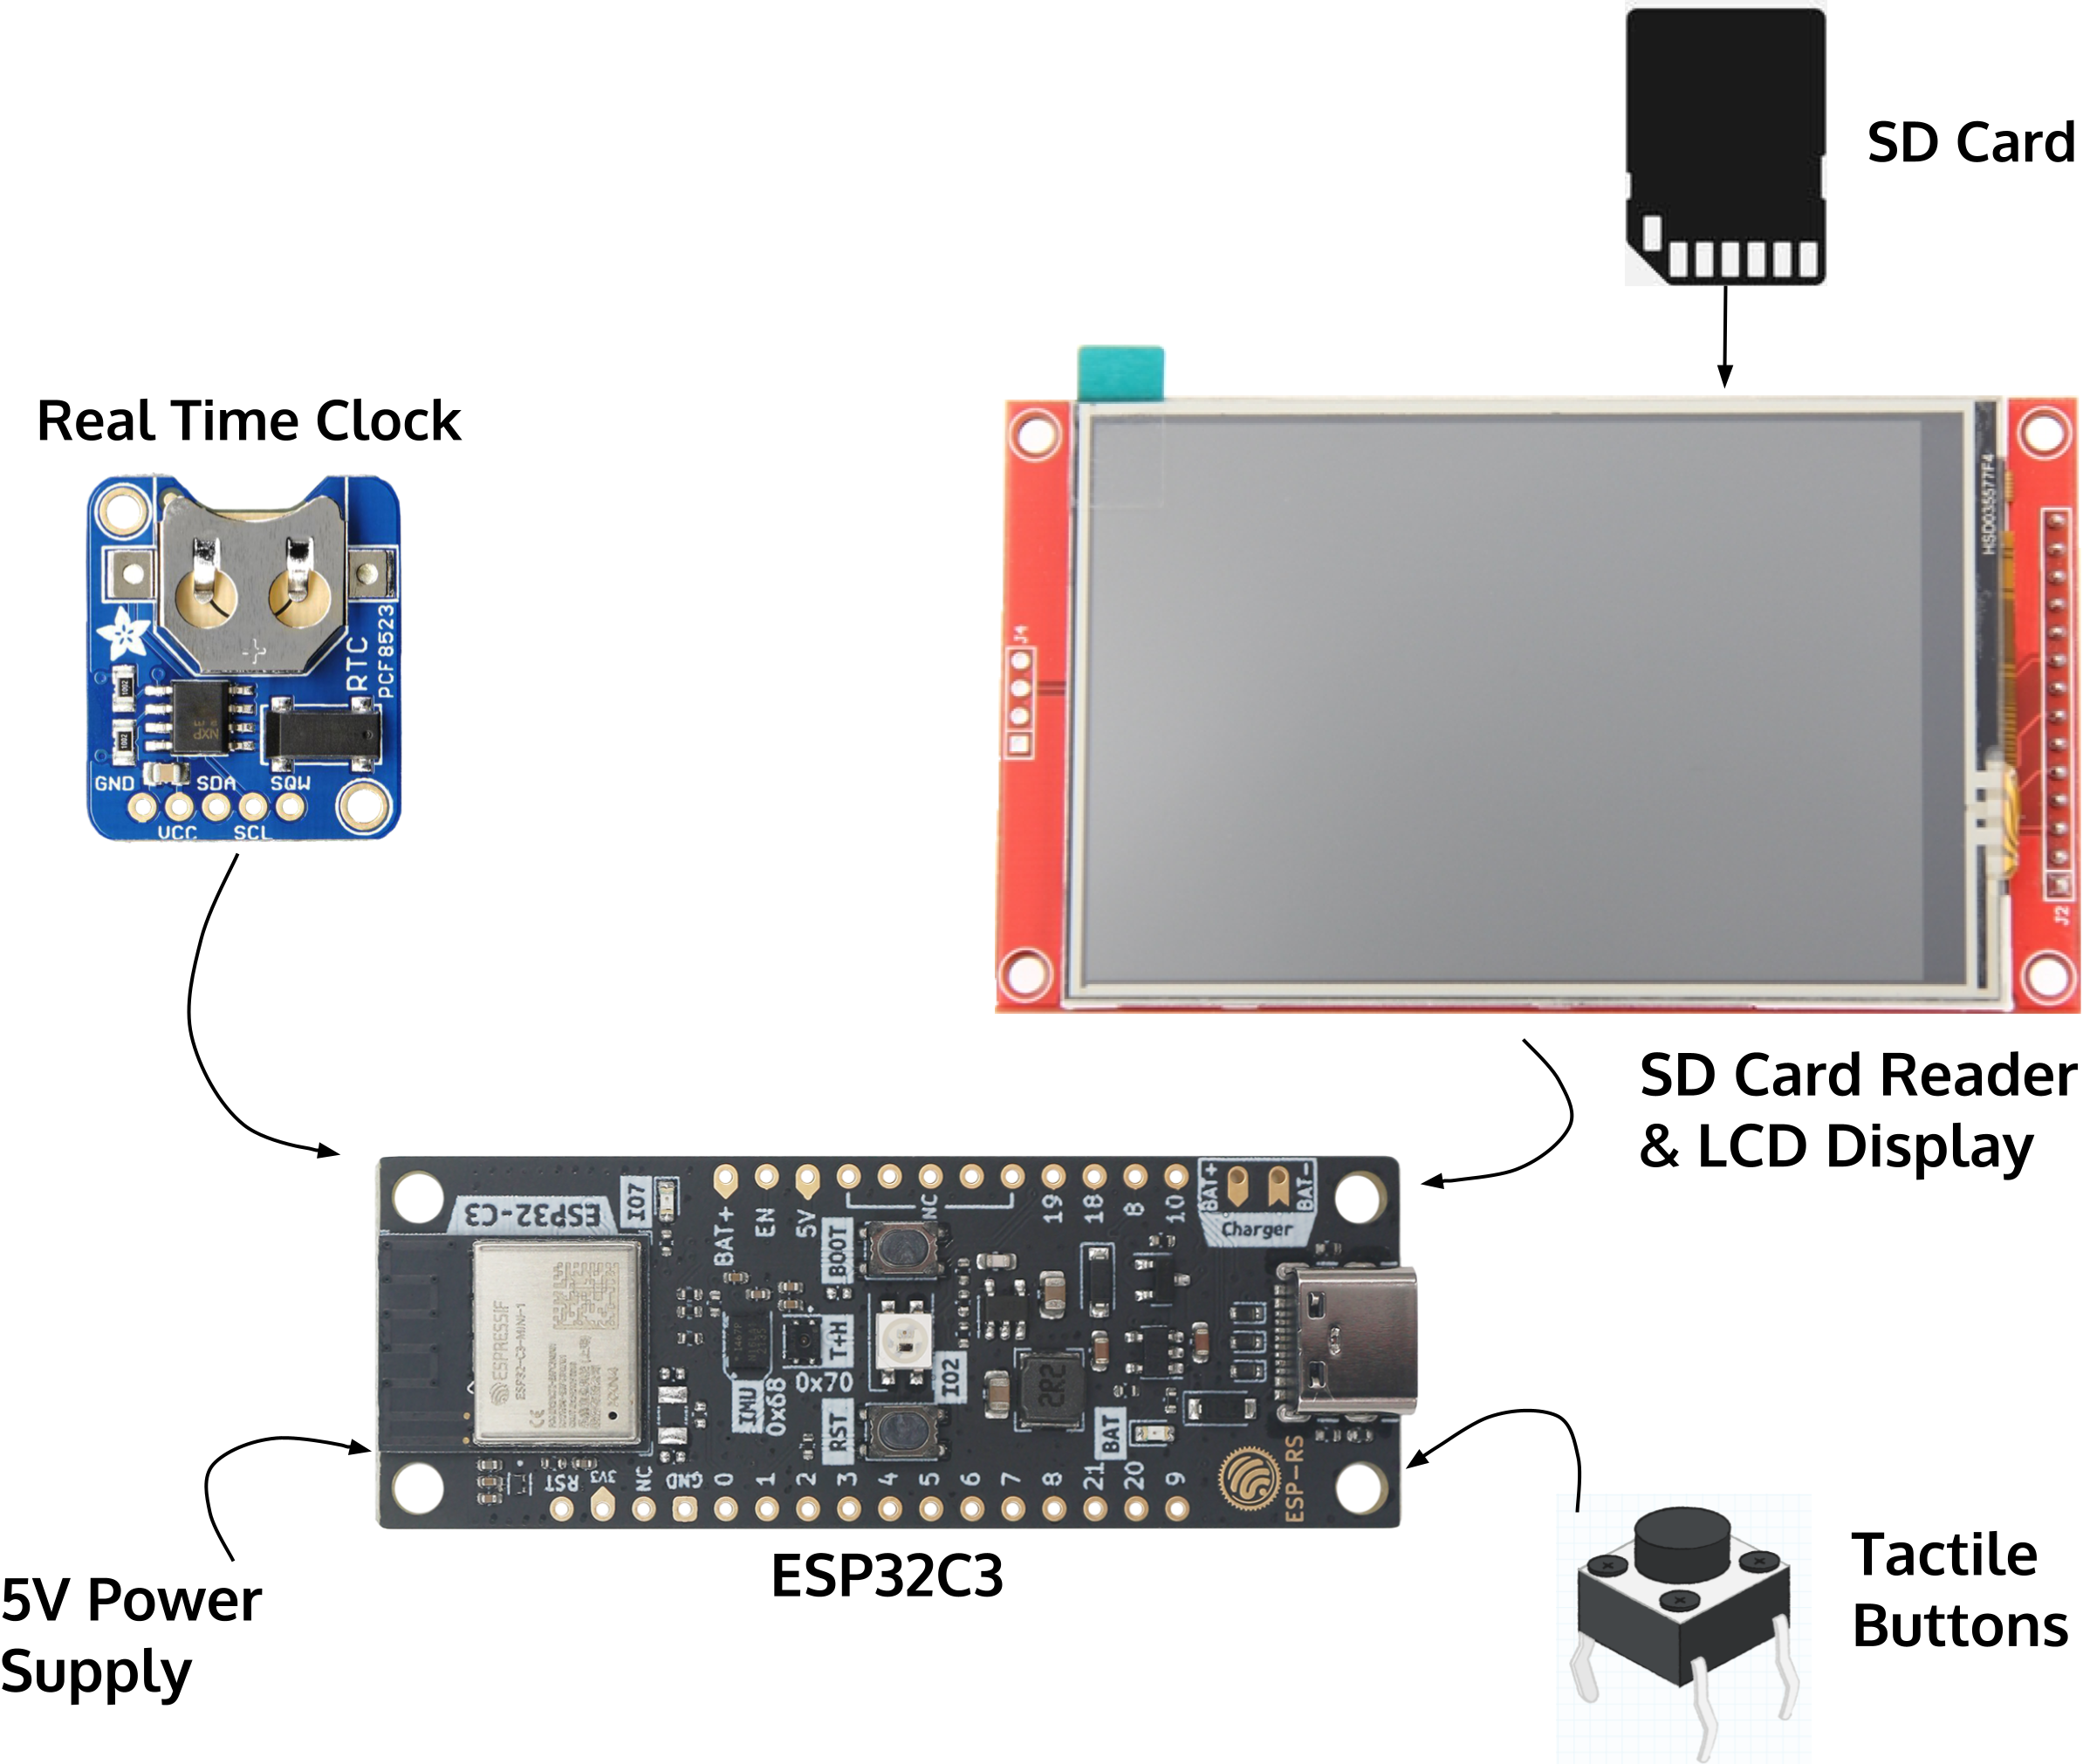
\includegraphics[width =\textwidth]{PrototypeDesign.png}
            \caption{Component Diagram}
        \end{subfigure}
        \begin{subfigure}[t]{0.44\textwidth}
            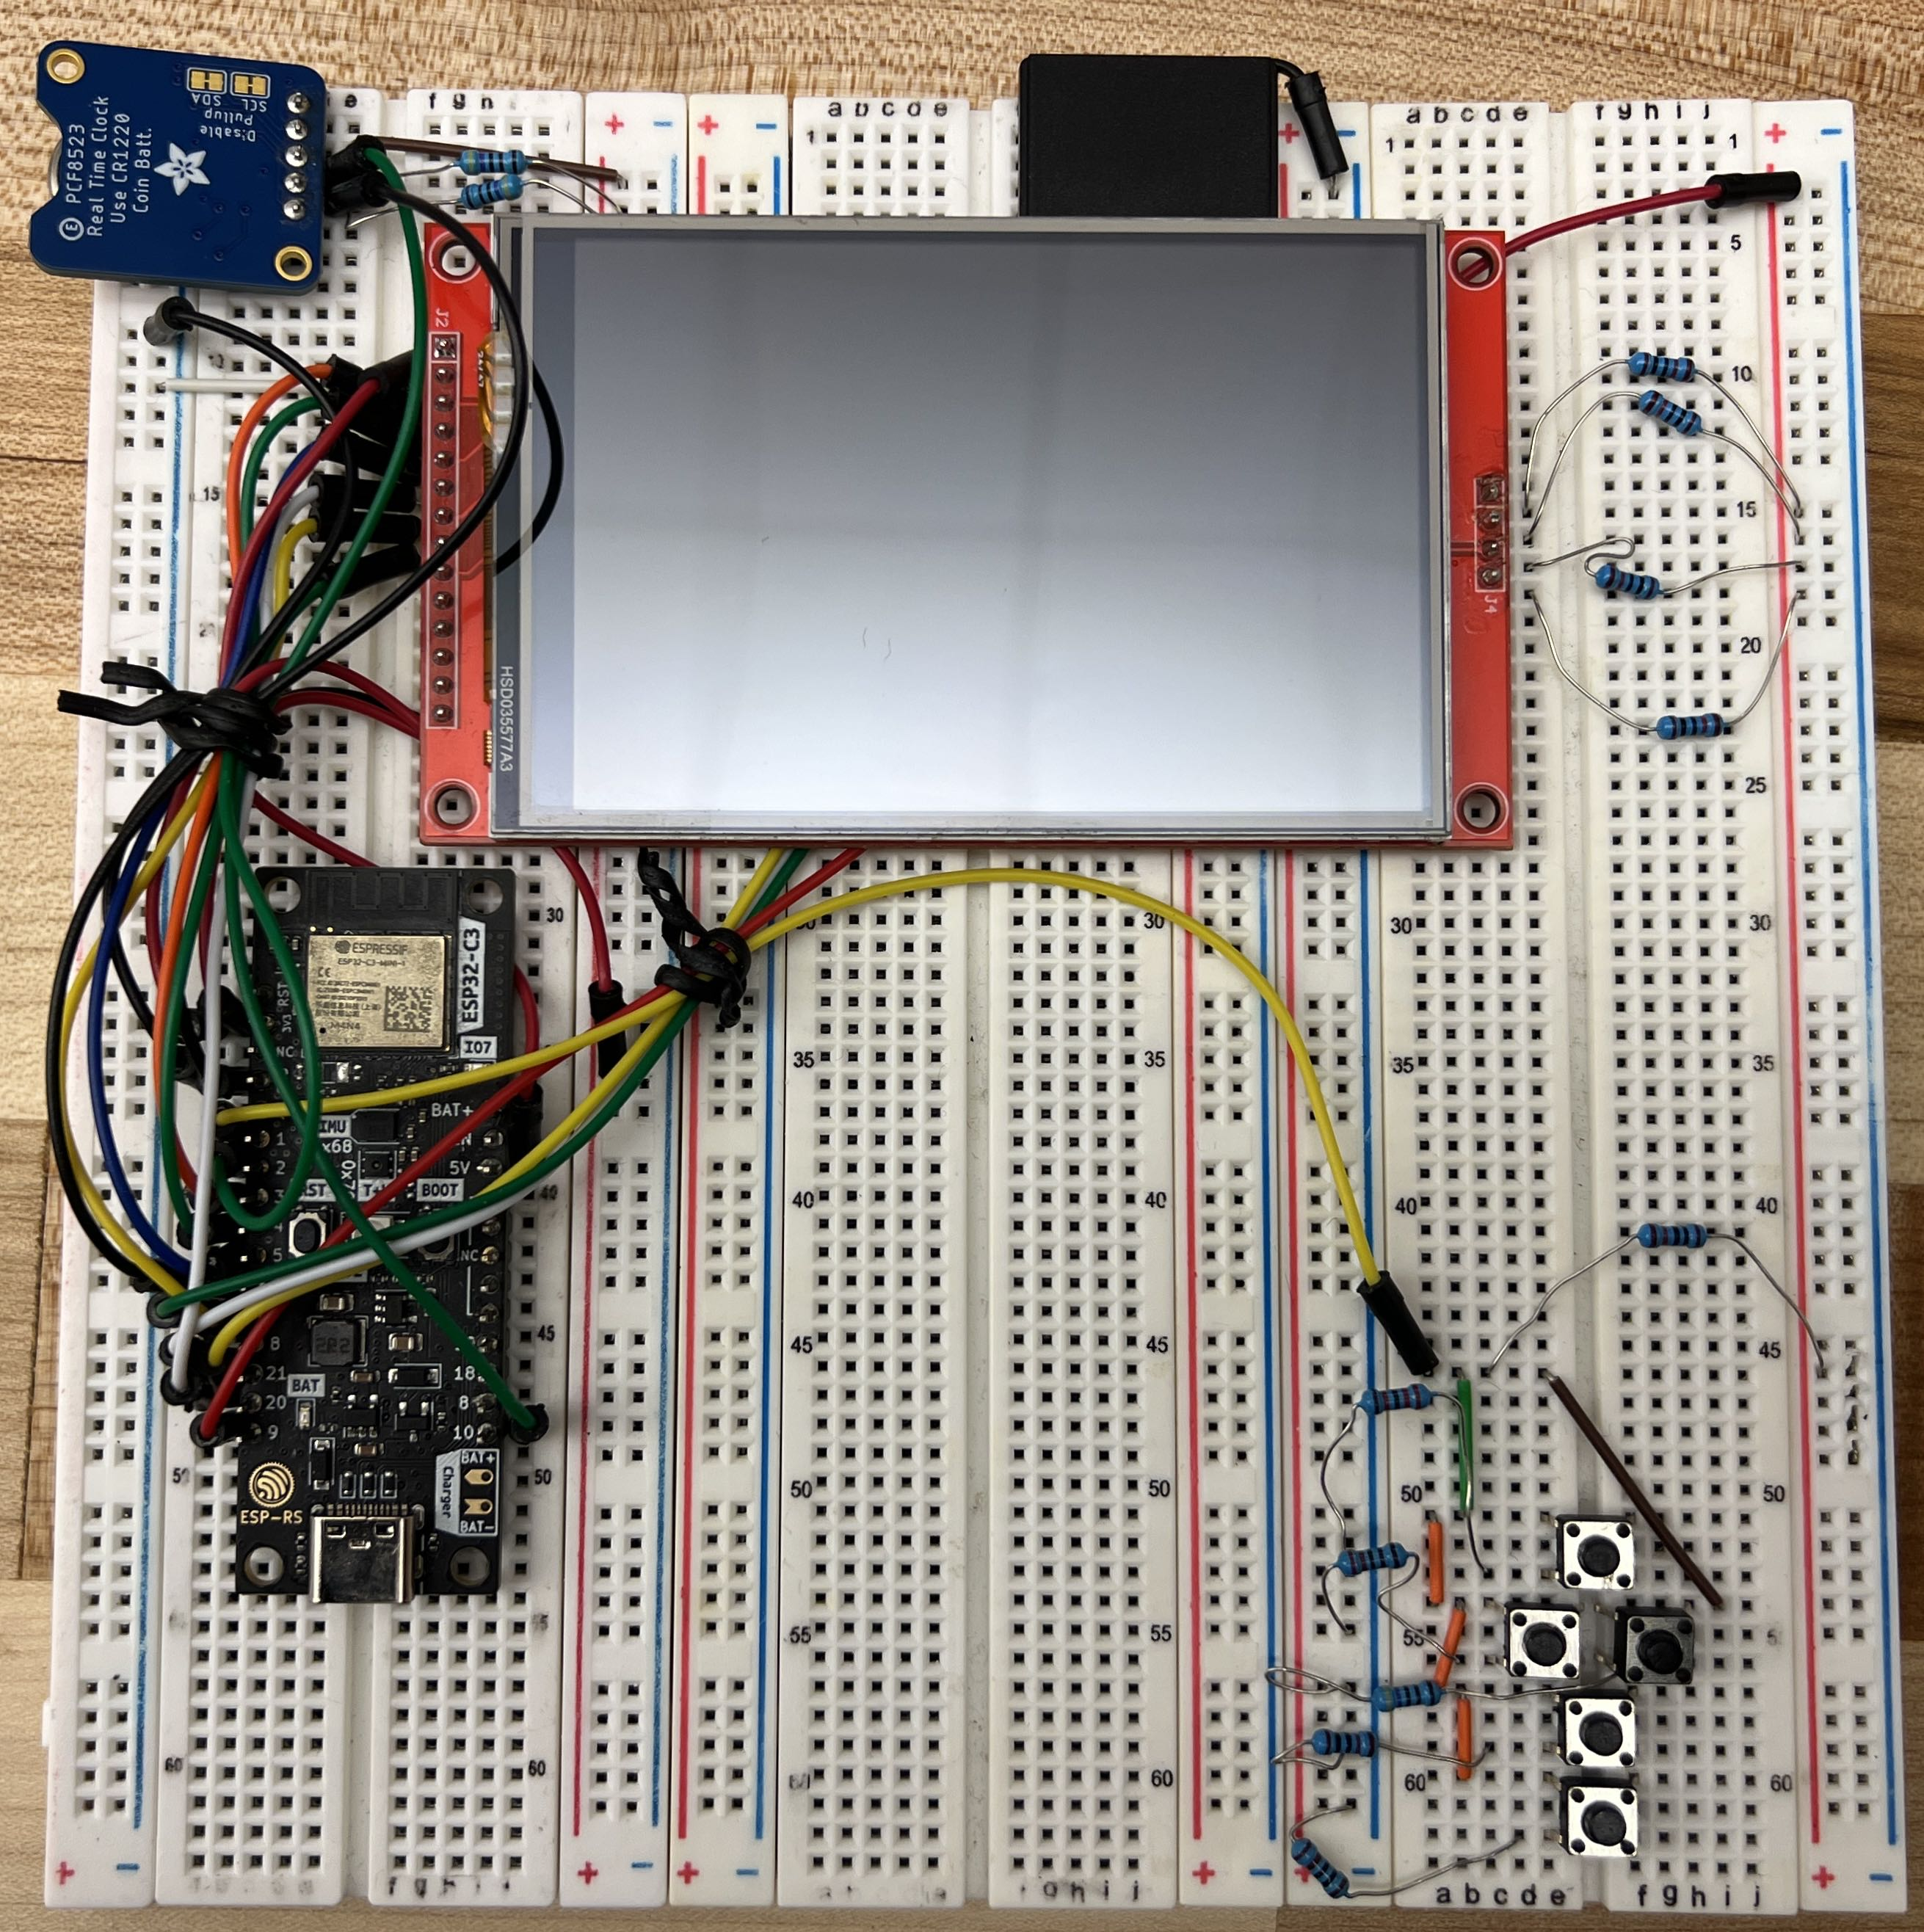
\includegraphics[width=\textwidth]{prototype.jpg}
            \caption{Functional Prototype}
        \end{subfigure}
      \end{figure}

        \begin{itemize}
          \item \textbf{Input}: Touch screen to navigate menus, edit data, and enter focus tasks.
          \item \textbf{Processing}: Custom microcontroller updates task database in real-time.
          \item \textbf{Display}: 3.5" LCD and webserver show current task/event list and status.
          \item \textbf{Storage}: RTC maintains devices track of time even when powered off, and the onboard SD card maintains all user data between resets.
        \end{itemize}

        Webapp allows user to edit activities and view calendar. Standalone device allows the user to view and mark their goals.

      \end{block}

      \begin{block}{Prototype Design}
        \textbf{Entries}

        To achieve their goals and maintain a healthy routine, device includes three tools to tackle the day:

        \begin{center}
          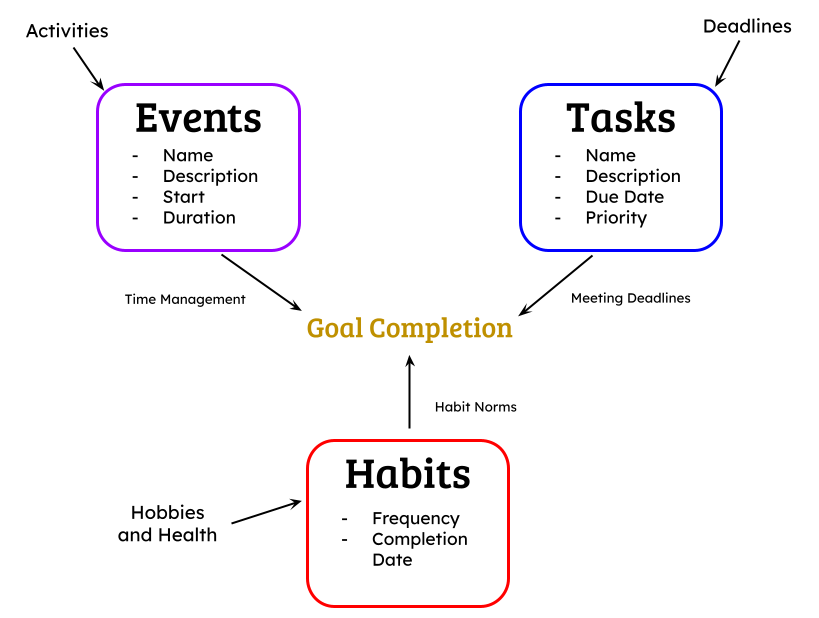
\includegraphics[width = 0.9 \textwidth]{entry_logic.png}
        \end{center}

        \textbf{Server-Client Modularization}

        Device works with strict limitations of ESP32C3 microcontroller while separating the user's computer from accurate display of user entires:

        \begin{enumerate}
          \item \textbf{Server Implementation} Users manage their data on the web server, producing entries that are accessible to their device.
          \item \textbf{Synchronization} Device periodically syncs by uploading local changes and retrieving server updates, prioritizing entry deletions.
        \end{enumerate}
      \end{block}

    \end{column}
    % ====================
    % End column 1
    % ====================

    \separatorcolumn

    % ====================
    % Begin column 2
    % ====================
    \begin{column}{\colwidth} 

      \begin{block}{User interface}
        \begin{figure}
          \centering
          \begin{subfigure}{0.49\textwidth}
            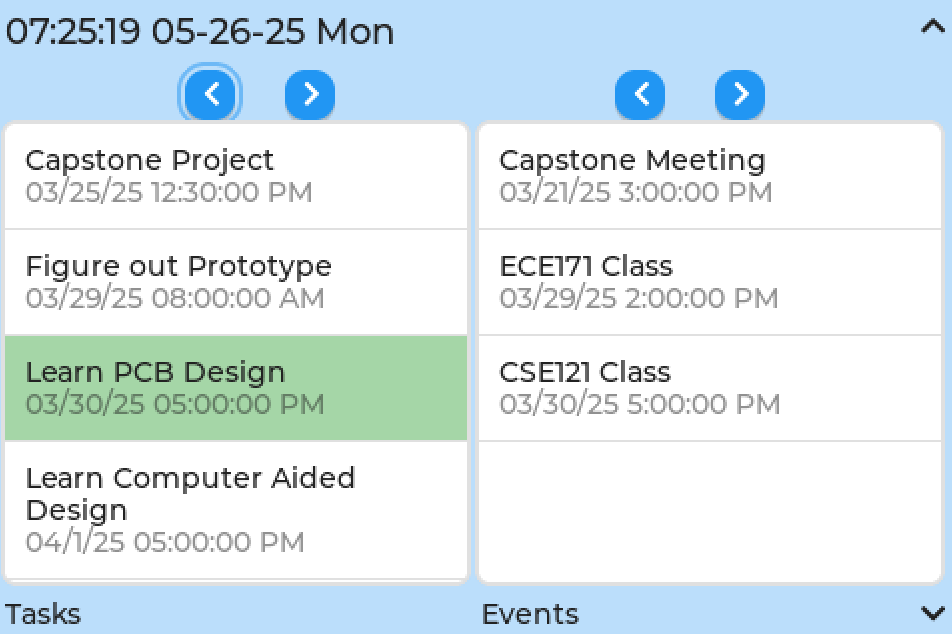
\includegraphics[width=\textwidth]{taskEvent.png}
            \caption{Main Menu}
          \end{subfigure}
          \hfill
          \begin{subfigure}{0.49\textwidth}
            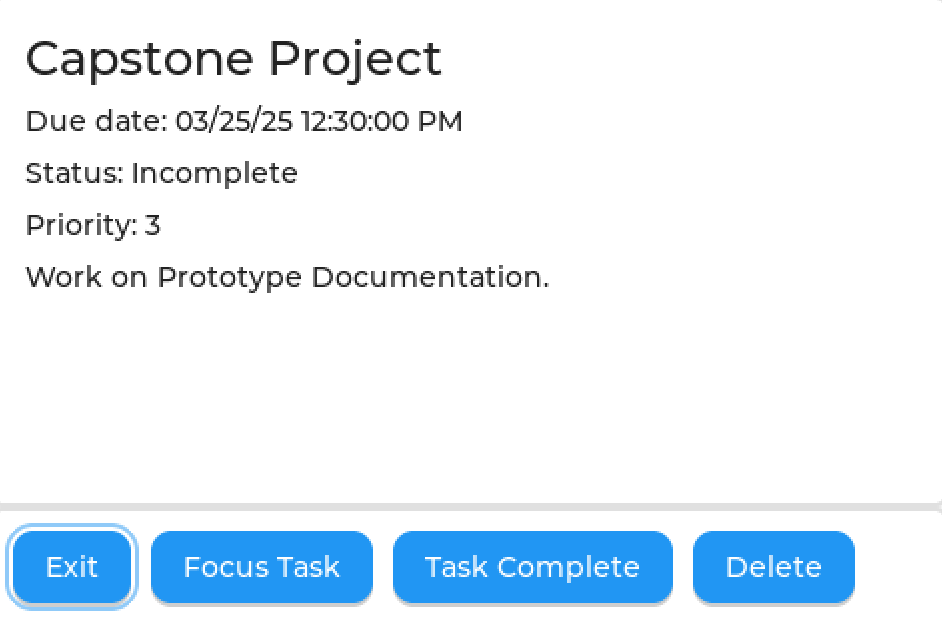
\includegraphics[width=\textwidth]{taskTile.png}
            \caption{Detailed Task View}
          \end{subfigure}
          \\
          \begin{subfigure}{0.49\textwidth}
            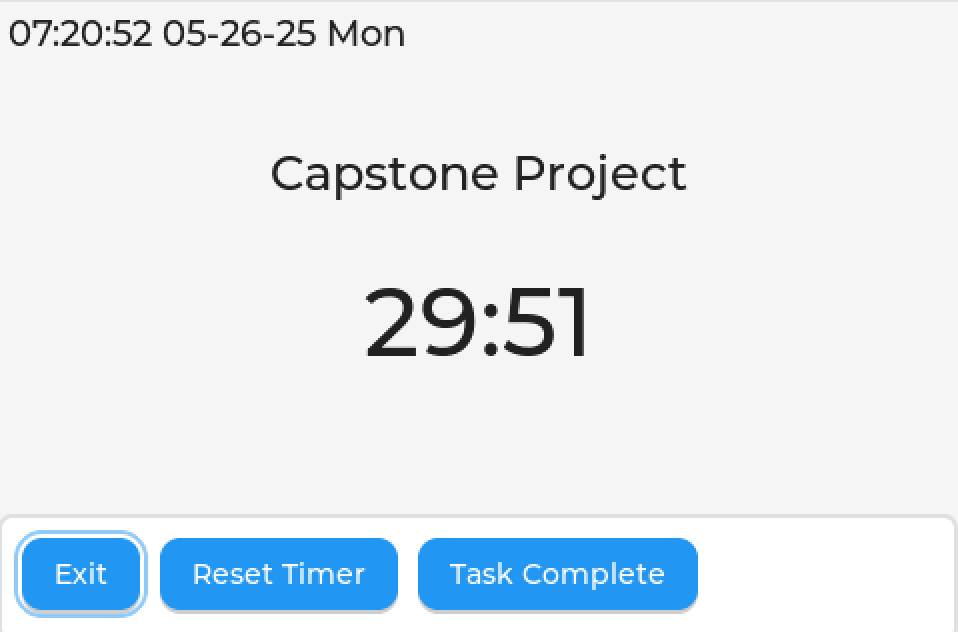
\includegraphics[width=\textwidth]{focusTile.png}
            \caption{Focus Task View}
          \end{subfigure}
          \hfill
          \begin{subfigure}{0.49\textwidth}
            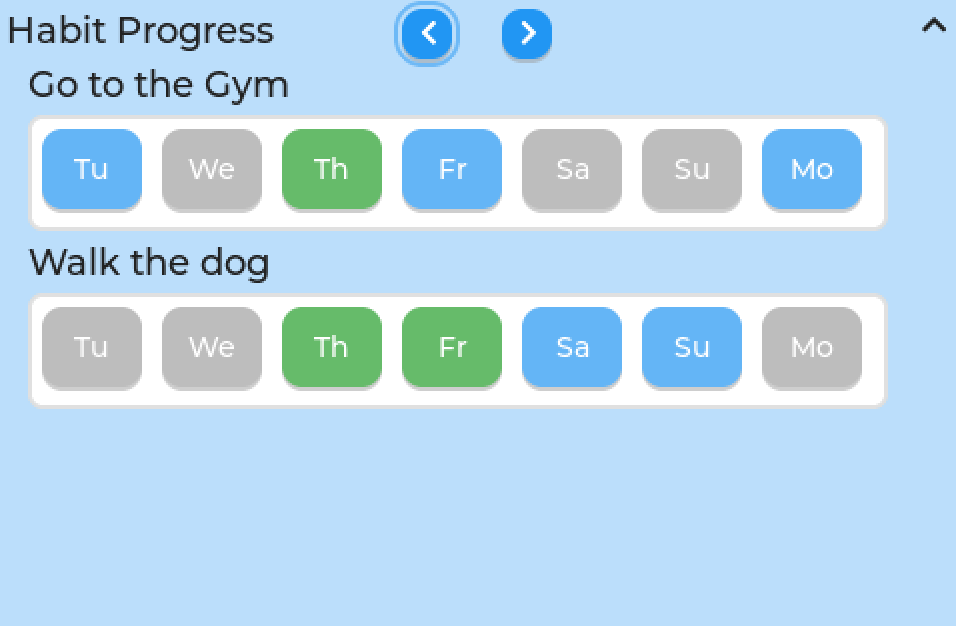
\includegraphics[width=\textwidth]{habitTile.png}
            \caption{Habit Tracking View}
          \end{subfigure}
        \end{figure} 
      \end{block}

      \begin{block}{Server Architecture}
        \vskip 0.5cm
        \begin{center}
          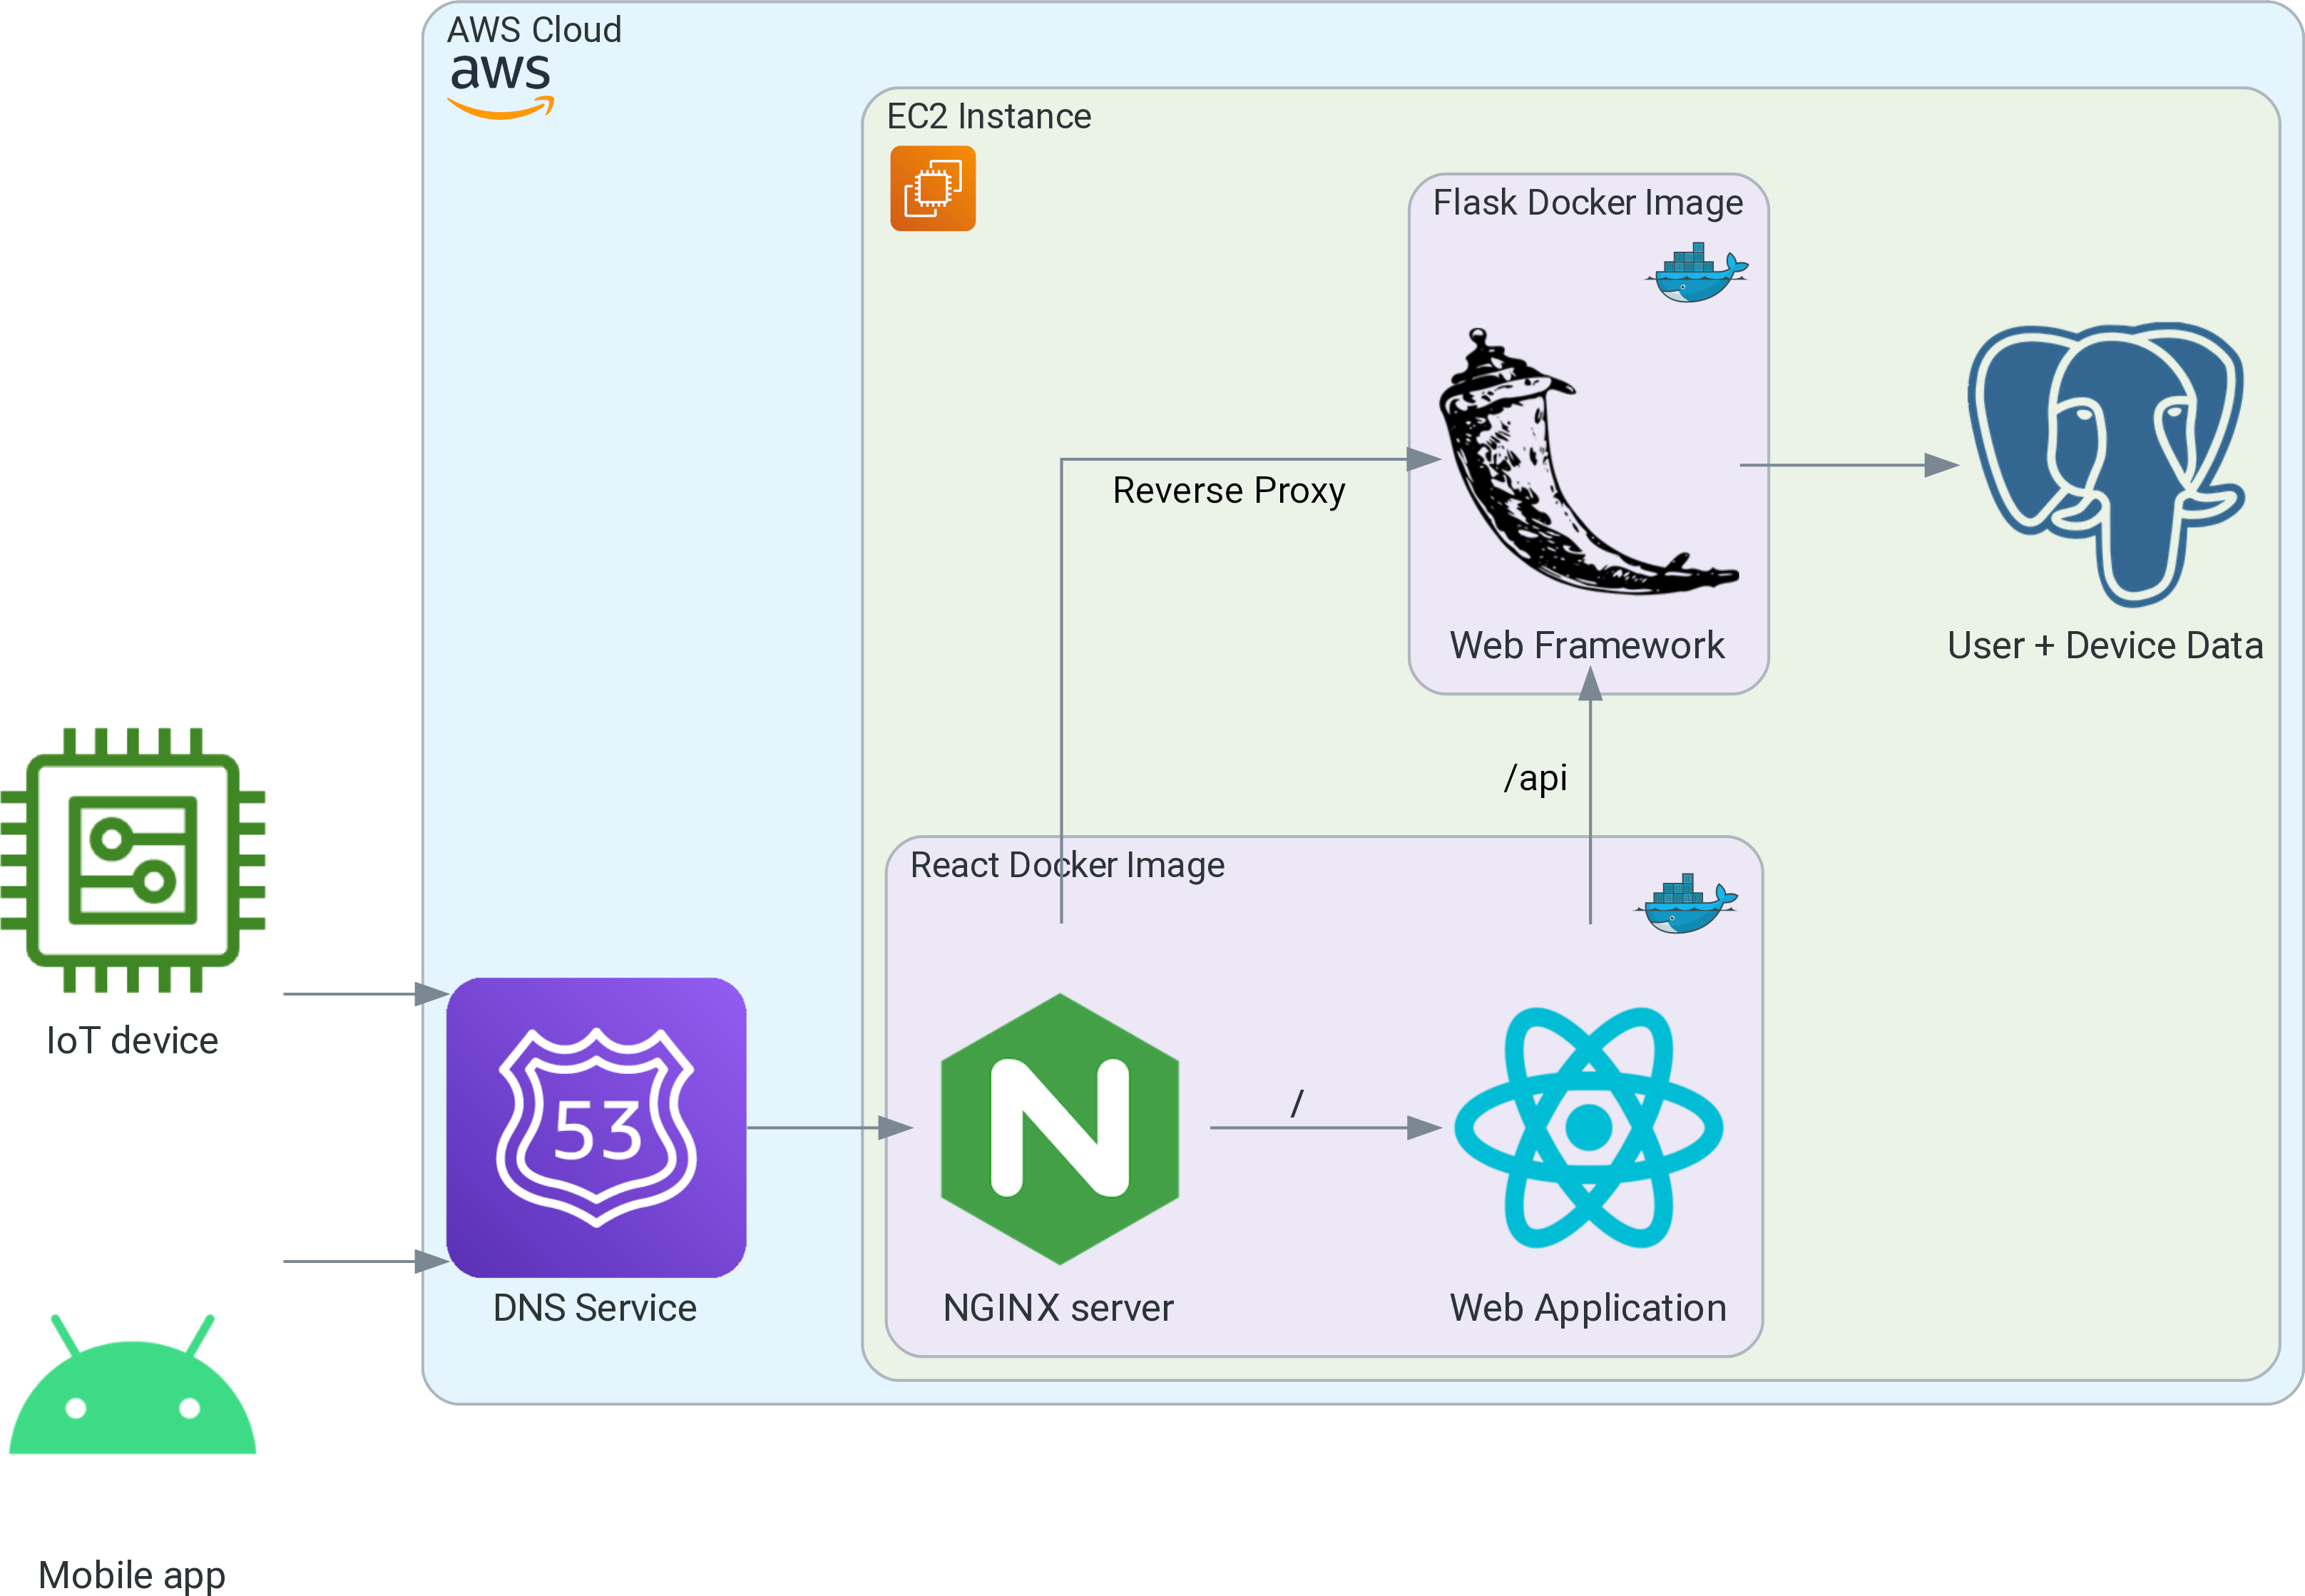
\includegraphics[width = \linewidth]{data_flow.png}
        \end{center}
      \end{block}

      \begin{block}{Web Interface}
        \begin{figure}
          \begin{subfigure}{\textwidth}
            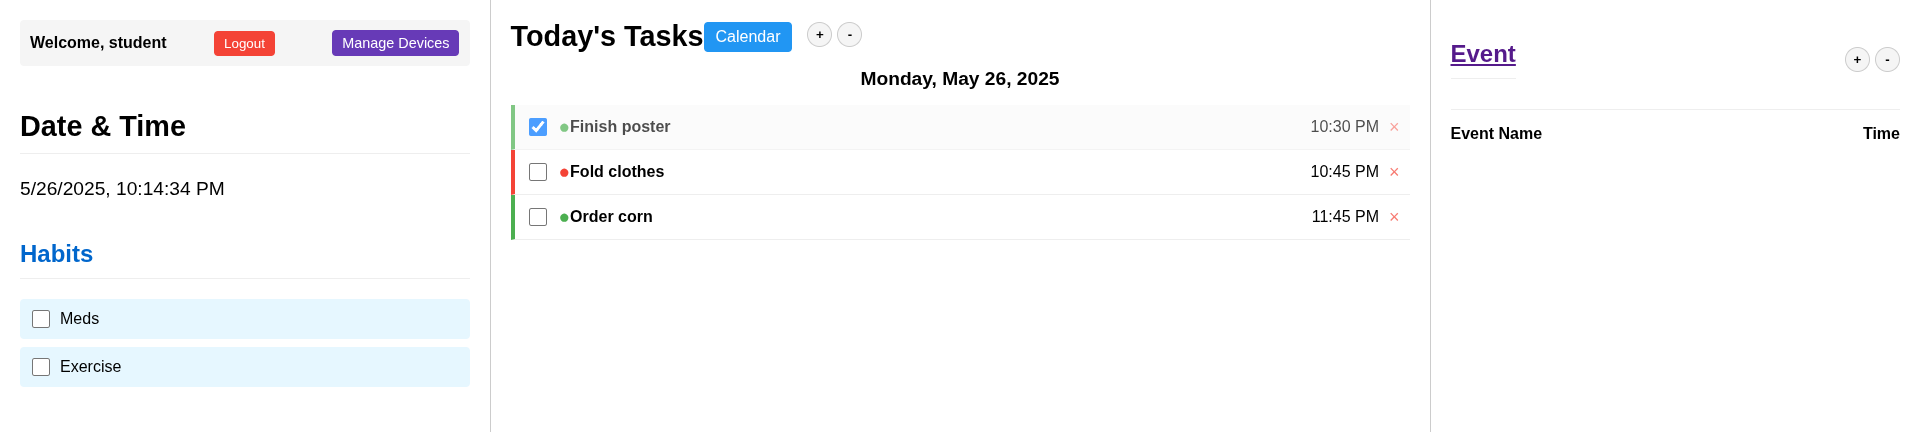
\includegraphics[width = \textwidth]{web_mainview.png}
            \caption{Home Page}
          \end{subfigure}
          \hfill
          \begin{subfigure}{0.49\textwidth}
            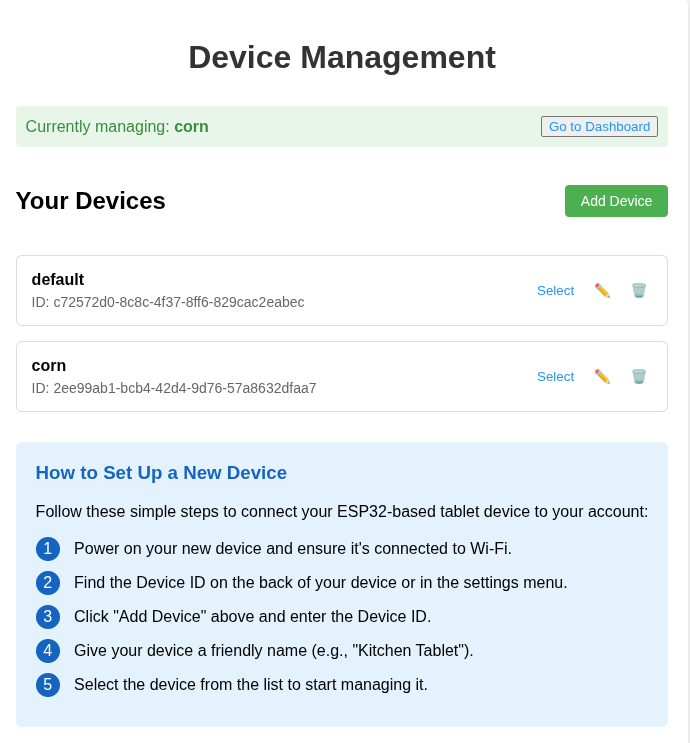
\includegraphics[width = \textwidth]{web_devices.png}
            \caption{Device Management}
          \end{subfigure}
        \end{figure}
      \end{block}

    \end{column}
    % ====================
    % End column 2
    % ====================

    \separatorcolumn

  \end{columns}
\end{frame}

\end{document}
